\chapter{A Medical Case Study}\label{c:medical-study}

In this thesis we primarly focus to analyze medical data by using some of the afforiomentioned techniques from section \ref{c:preliminaries}.
More specifically, we have developed algorithms for secure data aggregation and classification under the secure multi-party computation scenario.
In such a case, the computing nodes are not necessarily the ones that also provide the data.
Indeed, in our study, the data providers are hospitals and the computing nodes are three different servers.
When the medical data are transfered from the hospitals to the computing nodes, a secret sharing scheme is applied; Thus it is impossible for any of the three nodes to decrypt them, and in general to infer any information.
As we examined in section \ref{s:smpc}, the only requirement of the three computing parties is not to collude simultaneously.
An ideal way to prevent collusion, is to deploy them in premises with conflicting interests.


After gathering the patients' data, the computing nodes can evaluate any arbitrary function that is deployed with respect to the SMPC model.
% Any third party or analyst, can request 



\begin{figure}[H] 
  \centering
  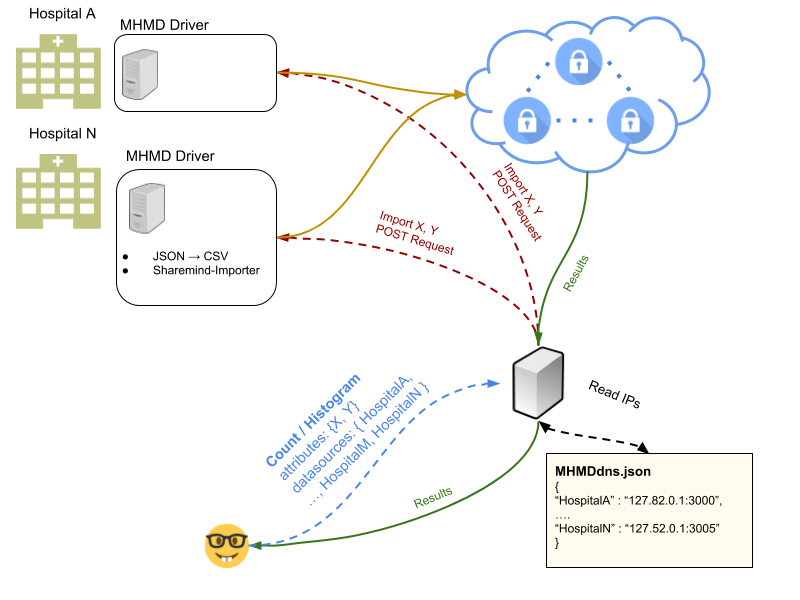
\includegraphics[width=\linewidth]{figures/overview.png}
  % \vspace{-0.2in}
  \caption{An overview of the architecture of our study}\label{f:overview}
\end{figure} 

